\setcounter{chapter}{2}
\setcounter{section}{0}
\part{FUNDAMENTACIÓN TEÓRICA DE LA INVESTIGACIÓN}

\section*{FUNDAMENTACIÓN TEÓRICA}
En este capítulo, se expondrán los trabajos relacionados con el presentado en este documento que se han identificado en la literatura, y que demuestran que el trabajo propuesto en este documento, aporta algo. Además se contextualiza el trabajo y define los términos novedosos y de poco dominio para los investigadores y para la comunidad.

\section{Marco referencial}

El diagrama de clases sin duda es el artefacto más importante para modelar un sistema y el punto de partida para otros diagramas \cite{Tan2010}. La problemática de la obtención de diagramas de clases a partir de los casos de uso detallados no ha sido tratada a profundidad. Por lo tanto los investigadores se encuentran en un campo fértil de investigación.

Las soluciones que se han propuesto y que se han recuperado en este trabajo, utilizan el procesamiento del lenguaje natural (NLP por sus siglas en inglés \textit{Natural Language Process}). Entre las soluciones encontradas podemos mencionar el trabajo de Chen y Zeng \cite{Chen2010}, en el cual presentan una aproximación sobre la obtención del diagrama de casos de uso y el diagrama de clases UML a partir de los requisitos del producto expresados en lenguaje natural. Sin embargo, en este trabajo intentan analizar el texto para determinar el conjunto de palabras significativas que pueden representar los elementos de los diagramas, por ejemplo, para una clase un sustantivo, para un método un verbo nominal para los métodos, la conexión entre dos objetos (clases) expresarían una relación. El trabajo de Chen \& Zeng \cite{Chen2010} tiene buenos resultados con pocos y bien establecidos requisitos de software, que pueden animar a los investigadores a seguir mejorando esa herramienta, como por ejemplo, identificar los diferentes tipos de relaciones entre clases, y su representación en el diagrama UML.

El trabajo presentado por Dawood Omer \& Eltyeb \cite{Dawood2022} es otra de las soluciones propuestas. En \cite{Dawood2022} proponen un modelo de razonamiento que basado en casos puede facilitar el proceso de generación de diagramas de clases UML a partir de requisitos textuales. Para ello utilizan técnicas de minería de texto. Por lo tanto el trabajo es bastante abrumador: primero se deben tener una base de casos para entrenar el modelo, luego se debe entrenar el modelo. Además, aunque las diferencias sean muy pequeñas, los resultados (diagrama de clases UML) puede variar.

En la misma línea de la aplicación de procesamiento del lenguaje natural para la obtención del diagrama de clases a partir de la descripción textual de los requisitos, podemos citar el trabajo de Abdelkareem M. Alashqar \cite{Alashqar2021}, en el que, para lograr este objetivo proponen un algoritmo y una herramienta. El algoritmo consiste básicamente en la separación de la oración en cada palabra que la conforman para luego aplicar un análisis morfológico a cada palabra, según el tipo de palabra (sustantivo, verbos en diferentes voces o tiempos, etc.) determinar los diferentes elementos de los diagramas. En este caso, la herramienta que implementan para aplicar el algoritmo muestra las oraciones que han sido mal escritas. Alshgar en su trabajo \cite{Alashqar2021} especifica que, para el algoritmo funcione correctamente, los requisitos textuales deben estar escritos con ciertas restricciones, como por ejemplo: cada oración debe estar escrita en una línea (separadas con un nueva línea), y que cada oración represente una acción a realizar con el software, entre otras restricciones. 

De los trabajos que se revisado hay que recalcar que \cite{Alashqar2021} y \cite{Shweta2020} se preocupan por el análisis de oraciones (acciones) pasivas negativas. Sin embargo todos los trabajos que utilizan NLP están limitados al idioma en el que están escritos los requisitos, y al uso correcto de la gramática y todos consideran restricciones en la escritura. Por lo que se presenta a Armadillo como una librería que ayuda que SymLen sea un lenguaje a utilizar para la escritura de los casos de uso detallados sin importar el idioma, y sin ninguna restricción. Con Armadillo la eficiencia de los diagramas de clases y la generación de código de software que satisface los requisitos del usuario, depende estrictamente del uso correcto de SymLen, y/o de la corrección de los posibles errores de su uso que Armadillo muestre al analista.

\section{Marco contextual}

En esta sección, se describe el entorno de trabajo investigativo realizado a este proyecto. Este marco complementa al resto de los referentes, que sirven de marco a una investigación.

\subsection{Metodología de desarrollo aplicada al proyecto}

Para llevar a cabo la ejecución del proyecto presentado, se analizo el Manifiesto por el Desarrollo Ágil de Software. La metodología aplicada a este proyecto se baso los Principios del Manifiesto Ágil. Con el objetivo de cumplir las directrices de una metodología ágil que permita realizar el proyecto de manera optima. En la tabla \ref{tab:analisis_principios} se redactan los 12 principios del manifiesto ágil y su aplicación en la metodología que se describiría en la siguiente sección. 

\begin{table}[]
	\centering
	\begin{tabular}{|l|l|}
		\hline
		\textbf{Principios del manifiesto ágil}                                                                                                                                                                                                  & \textbf{Análisis aplicado a la metodología}                                                                                                                                                                                               \\ \hline
		\textit{\begin{tabular}[c]{@{}l@{}}Nuestra mayor prioridad es satisfacer \\ al cliente mediante la entrega tempra-\\ na y continua de software con valor\end{tabular}}                                                                   & \begin{tabular}[c]{@{}l@{}}Para la entrega continua de cambios sobre \\ el desarrollo del script, se describieron va-\\ rias fases de desarrollo para ir cumpliendo \\ poco a poco los objetivos del trabajo pre-\\ sentado.\end{tabular} \\ \hline
		\textit{\begin{tabular}[c]{@{}l@{}}Aceptamos que los requisitos cambien, \\ incluso en etapas tardías del desarrollo. \\ Los procesos Ágiles aprovechan el \\ cambio para proporcionar ventaja com-\\ petitiva al cliente.\end{tabular}} &                                                                                                                                                                                                                                           \\ \hline
		\textit{\begin{tabular}[c]{@{}l@{}}Entregamos software funcional frecuen-\\ temente, entre dos semanas y dos meses, \\ con preferencia al periodo de tiempo \\ más corto posible.\end{tabular}}                                          &                                                                                                                                                                                                                                           \\ \hline
		\textit{\begin{tabular}[c]{@{}l@{}}Los responsables de negocio y los desa-\\ rrolladores trabajamos juntos de forma\\  cotidiana durante todo el proyecto.\end{tabular}}                                                                 &                                                                                                                                                                                                                                           \\ \hline
		\textit{\begin{tabular}[c]{@{}l@{}}Los proyectos se desarrollan en torno a \\ individuos motivados. Hay que darles \\ el  entorno y el apoyo que necesitan, \\ y confiarles la ejecución del trabajo.\end{tabular}}                      &                                                                                                                                                                                                                                           \\ \hline
		\textit{\begin{tabular}[c]{@{}l@{}}El método más eficiente y efectivo \\ de comunicar información al equipo \\ de desarrollo y entre sus miembros \\ es la conversación cara a cara.\end{tabular}}                                       &                                                                                                                                                                                                                                           \\ \hline
		\textit{\begin{tabular}[c]{@{}l@{}}El software funcionando es la medida\\ principal de progreso\end{tabular}}                                                                                                                            &                                                                                                                                                                                                                                           \\ \hline
		\begin{tabular}[c]{@{}l@{}}Los procesos Ágiles promueven el de-\\ sarrollo sostenible. Los promotores, \\ desarrolladores y usuarios debemos ser \\ capaces de mantener un ritmo constante \\ de forma indefinida.\end{tabular}          &                                                                                                                                                                                                                                           \\ \hline
		\textit{\begin{tabular}[c]{@{}l@{}}La atención continua a la excelencia \\ técnica y al buen diseño mejora \\ la Agilidad.\end{tabular}}                                                                                                 &                                                                                                                                                                                                                                           \\ \hline
		\textit{\begin{tabular}[c]{@{}l@{}}La simplicidad, o el arte de maxi-\\ mizar la cantidad de trabajo no \\ realizado, es esencial.\end{tabular}}                                                                                         &                                                                                                                                                                                                                                           \\ \hline
		\textit{\begin{tabular}[c]{@{}l@{}}Las mejores arquitecturas, requisitos \\ y diseños emergen de equipos \\ auto-organizados.\end{tabular}}                                                                                              &                                                                                                                                                                                                                                           \\ \hline
		\textit{\begin{tabular}[c]{@{}l@{}}A intervalos regulares el equipo \\ reflexiona sobre cómo ser más \\ efectivo para a continuación \\ ajustar y perfeccionar su \\ comportamiento en consecuencia.\end{tabular}}                       &                                                                                                                                                                                                                                           \\ \hline
	\end{tabular}
	\caption{Análisis de los principios ágiles en la metodología aplicada.}
	\label{tab:analisis_principios}
\end{table}

\subsubsection{Descripción general de la metodología}

Esta metodología consta de 5 fases. Aparentemente agrupan fases que estén relacionadas al desarrollo de un sistema, desde el análisis de requisitos hasta su debido mantenimiento. Esta última es muy olvidada por los investigadores, y es de mucho interés en la vida de desarrollo. En la figura \ref{fig:metod} se pueden observar las fases que deben eser implementadas para utilizar la metodología redactada.

\begin{figure}[h!]
	\centering
	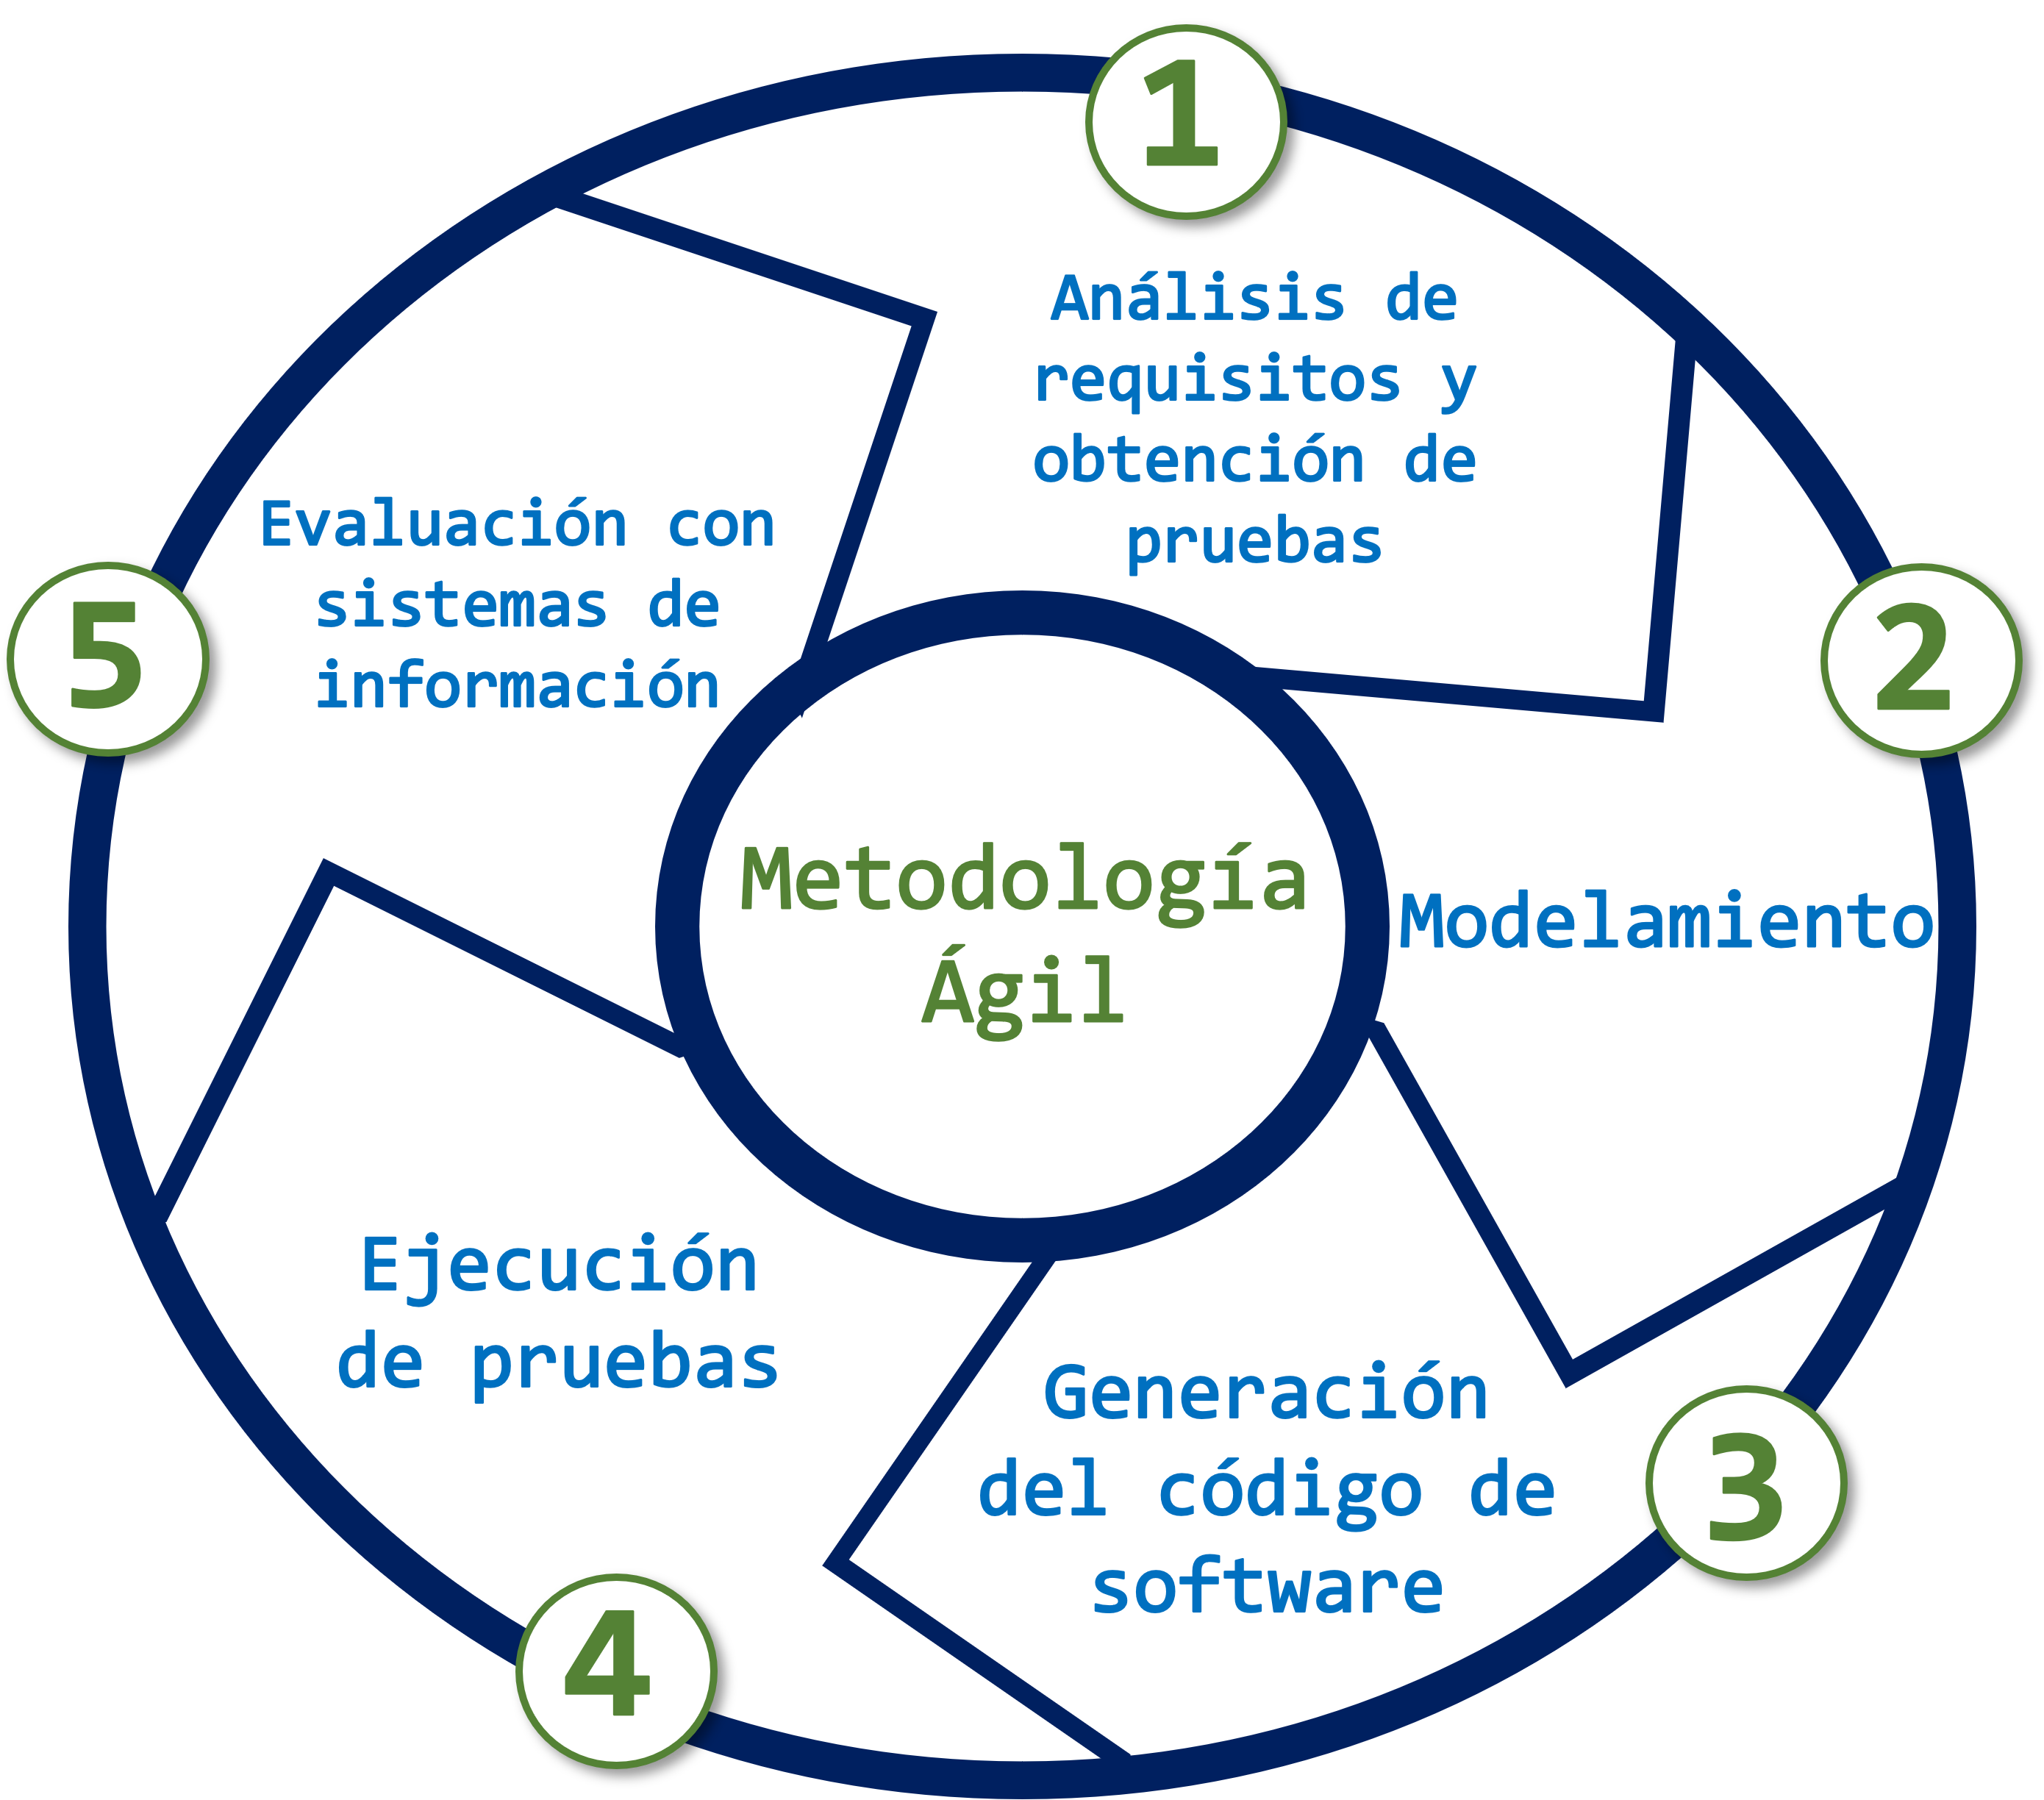
\includegraphics[width=10cm]{img/metodologia.png}
	\caption{Fases de la metodología. \\ ELABORADO: Carvajal Suárez Dúval}
	\label{fig:metod}
\end{figure}

Las principales razones del uso de una metodología ágil es el uso de un ciclo de desarrollo iterativo e incremental para la ejecución de este proyecto son:

\begin{itemize}
	\item Entregas frecuentes y continuas de forma que puede disponer de una funcionalidad básica en un tiempo mínimo y a partir de ahí un incremento y mejora continua del sistema.
	
	\item Previsible inestabilidad de requisitos. Es posible que el sistema incorpora más funcionalidades de las inicialmente identificadas
	
	\item Es posible que durante la ejecución del proyecto se altere el orden en el que se desean recibir los módulos.
\end{itemize} 

Para mejorar la ejecución de la metodología se organizaron diferentes tipos de roles que deben ser tomados por las personas que desarrollen del proyecto. Cada rol implementado juega un papel muy importante dentro de la metodología, debido a que deben cumplir tareas de suma importancia para controlar todas las fases que se deben seguir y cumplir los objetivos del trabajo a desarrollar.

\paragraph{Roles}

El equipo de esta metodología está conformado por 2 roles, Director de proyecto (DP) y el Desarrollador de Sistemas (DS). Todos los miembros de un equipo de desarrollo tienen diferentes roles en la gestión y supervisión de los proyectos. Todos los roles son necesarios para que el proceso funcione eficientemente. 

\begin{itemize}
	\item \textbf{Director de proyecto (DP):} Se encarga de administrar el proceso del proyecto, su planificación, coordinación con el analista y realizar un seguimiento e informes del progreso del proyecto, en términos de calidad, costo y plazos de entrega. El DP es la interfaz principal entre el propietario del producto y el analista de desarrollo de software.
	
	\item \textbf{Desarrollador de Sistemas (DS):} La persona encargada de este rol debe contar con conocimientos de desarrollo de software. El desarrollador deberá estar totalmente familiarizado con el objetivo principal del trabajo. Debido a que sera el encargado de analizar todos los requisitos que se necesiten para cumplir con el funcionamiento optimo del sistema, también se encargara analizar, diseñar y codificar el producto final del proyecto.
	
	\begin{itemize}
		\item Comprometerse al inicio de cada modulo y desarrollar todas las funcionalidades en el tiempo determinado.
		
		\item Son responsables de entregar un producto a cada término de un modulo.
		
		\item Definir el desarrollo del sistema.
	\end{itemize} 
\end{itemize}

\paragraph{Fases}

En esta sección se describen cada una de las fases que se mencionaron en el apartado anterior, también se mencionaran breves conceptos relacionados a cada fase y como pueden mitigar los problemas que se pueden presentar a lo largo de la ejecución de la metodología redactada. 

\begin{enumerate}
	\item \textbf{Análisis de requisitos y obtención de pruebas:} Para la recopilación de los requisitos del software es necesario comprenderlos en profundidad para asegurar su correcto funcionamiento cuando este desarrollado. Si al momento de recopilar la información, no lleva todo el tiempo suficiente para ser analizado correctamente podría afectar todo el proyecto en general [1].
	
	Para que los requisitos obtenidos sean realizados de manera correcta se pueden priorizar. Existen técnicas actuales para realizar la priorización de requisitos como es el Proceso de Jerarquía Analítica (AHP) ya que produce resultados muy precisos. A continuación se especifican  tres tipos de técnicas de priorización [1]:
	
	\begin{itemize}
		\item \textit{Escala nominal: } El personal de trabajo que recopilo los requisitos, deberán asignar cada requisito a un grupo de prioridad, transformando a todos los requisitos de ese grupo prioritarios. La asignación numérica, categoriza los requisitos en grupos. Caga grupo cuenta con un identificador único que les permite ser identificados dentro de los demás grupos. 
		\item \textit{Escala ordinal: } Esta técnica produce una lista de requisitos y cada uno cuenta con una prioridad en especifica. Existe una técnica similar a la de escala nominal que se basa en crear varios grupos de prioridad. Pero solo son 3 tipos de grupos: alto, medio y bajo, los desarrolladores priorizan y clasifican los requisitos dentro del mismo grupo en otro subgrupo; ese bucle se repite hasta que cada grupo tenga sólo uno.
		\item \textit{Escala de relación: }Son similares a la escala ordinal, ademas muestran importancia relativa entre todos los requisitos, es decir que dan valores de prioridad a los requisitos.	En estas técnicas, los desarrolladores conocen hasta qué punto cada requisito es más importante que el resto. La votación acumulativa (CV) es una técnica proporcional que depende de la votación de los desarrolladores; cada desarrollador tiene 100 puntos y se distribuyen entre los requisitos en función de su prioridad 
	\end{itemize}
	
	La obtención de pruebas se basa en la recolección de los posibles escenarios que puedan ocurrir al momento consumir el producto final del proyecto. Ademas se necesita conocer el resultado que se deberá obtener por los parámetros ingresados por cada prueba. 
	 
	\item \textbf{Modelamiento: } El modelado de software básicamente son las abstracciones que describen la arquitectura de un sistema informático. Para llevar a cabo la ejecución de esta fase es necesario tener conocimientos sólidos sobre el desarrollo de software, debido a que los modelos pueden tener diferentes niveles de abstracción y detalles. 
	
	En [2] se propone un metamodelo que permite representar al software a base de patrones de diseño. Es decir se pueden crear diferentes tipos de diagramas personalizados especificando el comportamiento que tendrá el sistema informático cuando este en ejecución. Ademas se pueden vincular los patrones encontrados con pruebas de aceptación con los usuarios que usaran el producto final del proyecto presentado. 
	
	\item \textbf{Generación de código:} En la fase de generación de código se relaciona con obtener el producto o software de manera real. En esta etapa los desarrolladores deberán cumplir con algunos puntos claves en el desarrollo de software que son: personalizar la interfaz de usuario, implementar la lógica comercial, integrar servicios de terceros si es necesario o resolver problemas de desarrollo muy complejos que requieran un análisis mas profundo para llegar a una solución optima.
	
	Se recomienda a los encargados de ejecutar esta etapa tener conocimientos de programación. En [3] mencionan que si la curva de aprendizaje de los desarrolladores es baja, no necesitan obtener conocimientos al momento de generar el código del software. Esto permitirá suponer que el nivel de conocimiento puede impactar en el proceso de aprendizaje y adopción de la tecnología. 
	
	Ademas para suprimir un poco los grandes desafíos a los que se enfrentan los desarrolladores en este fase, se recomienda el uso de tecnologías con una documentación detallada y cuenten con recursos de aprendizaje. Otra solución potente para ayudar a los desarrolladores es basarse en un sistema similar al que se pretende desarrollar usando el conocimiento de aplicaciones previamente desarrolladas.  
	
	\item \textbf{Ejecución de pruebas:} La siguiente fase esta relacionada con la primera. Como se podrá observar en los títulos de estas dos fases, se realiza la obtención y ejecución de pruebas sobre el software que se obtendrá. Existen varios problemas que surgen al momento de poner en producción un software desarrollado. En [4] muestran varios estudios que indican que algunos tipos de fallos son intrínsecamente difíciles si no imposibles de detectar en entornos de desarrollo.
	
	Utilizando las pruebas de campo se puede realizar la manipulación del sistema teniendo a la mano los resultados esperados por los datos que son ingresados como entrada sobre el software. Es decir en esta fase se debe utilizar los datos que fueron recopilados en la primera fase y ser ingresados en el sistema que ya se encuentra totalmente desarrollado. Con el fin de obtener resultados similares o precisamente los mismos a los resultados obtenidos inicialmente.
	
	\item \textbf{Evaluación con sistemas de información:} La fase final de la metodología redactada permitirá usar sistemas de información ya desarrollados que permitan utilizar el producto final del proyecto ejecutado. Se recomienda utilizar sistemas de información con su documentación totalmente detallada, de esa manera se ahorra tiempo en analizar por completo los trabajos para ingresarlos al sistema informático que se desarrollo con esta metodología.
	
	
\end{enumerate}

\section{Marco conceptual}

En esta sección, se detalla los modelos teóricos, conceptos, argumentos o definiciones que se han desarrollado o investigado en relación con el tema en particular.


\subsection{Lenguajes de marcado}	

A continuación se describen una serie de formatos de texto utilizados para el intercambio de datos entre varias aplicaciones.

\subsubsection{JSON}

Javascript Object Notation (JSON) es un formato ligero de intercambio de datos. Consisten en asociación de nombres y valores. A pesar de ser independiente del lenguaje de programación, es admitido en una gran cantidad de lenguajes de programación. Se basa en un subconjunto del Estándar de lenguaje de programación JavaScript \cite{JSON}.

\begin{figure}[h!]
	\centering
	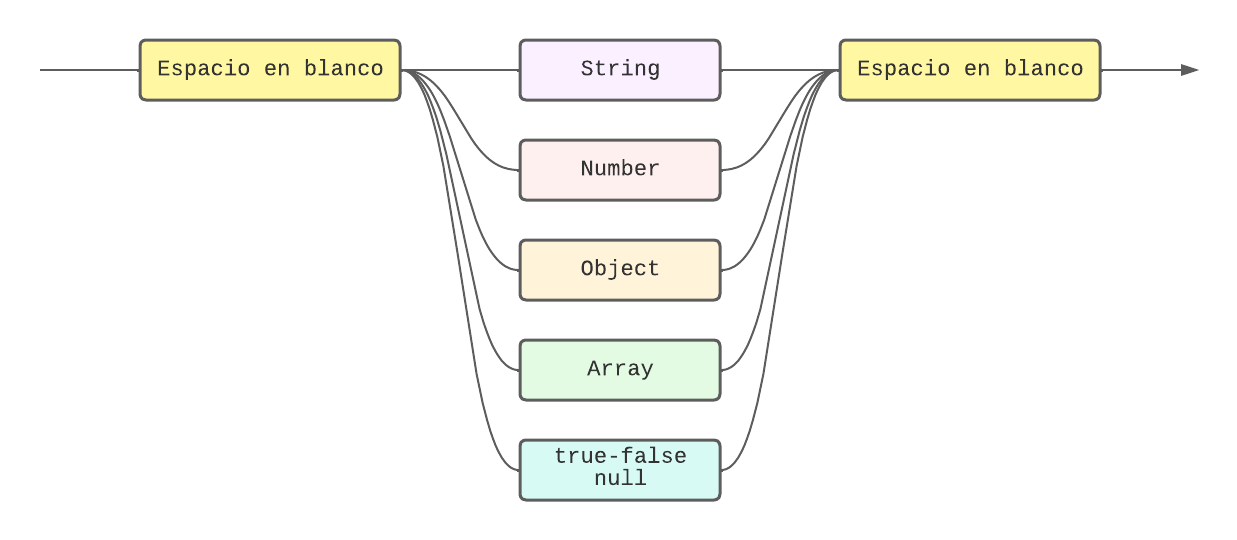
\includegraphics[width=12cm]{img/json.png}
	\caption{Estructura json.}
	\label{fig:json}
\end{figure}

\subsubsection{XML}

Es un lenguaje de marcado similar a HTML. Significa Extensible Markup Language y pertenece a la especificación W3C como lenguaje de marcado de propósito general. Esto significa que, a diferencia de otros lenguajes de marcado, XML no está predefinido, por lo que debe definir su propio marcado. El objetivo principal del lenguaje es compartir datos entre diferentes sistemas, como Internet \cite{XML-based}.

\begin{figure}[h!]
	\centering
	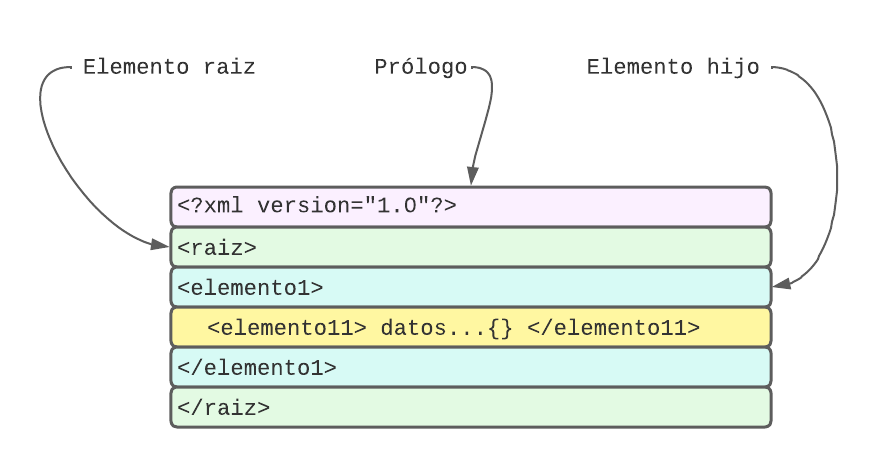
\includegraphics[width=12cm]{img/xml.png}
	\caption{Estructura xml.}
	\label{fig:xml}
\end{figure}

\subsection{Compiladores}
Están diseñados para traducir un fragmento de código escrito en un de lenguaje de programación a lenguaje de máquina que es, el que puede entender la computadora. El compilador analiza el código fuente en busca de errores antes de la traducción. Si se detecta un error, el compilador
notificar al autor del código para que pueda arreglarlo.. Además, los compiladores modernos o entornos de desarrollo (IDE), puede sugerir soluciones para algunos tipos de errores usando métodos de corrección de errores \cite{CoEdit}.

\subsection{Modelamiento de software}
Representan una serie de requisitos basados en la construcción de elementos visuales para definir estructuras y comportamientos que tendrá el software. UML (Lenguaje Unificado de Modelado) a través del mecanismo de perfilado, se han basado históricamente en notaciones gráficas. UML mediante el mecanismo de perfiles, maximiza la comprensión humana y facilita la comunicación entre las partes interesadas como son el cliente y desarrollador \cite{Blended}. 

También existen lenguajes de modelado personalizados para distintas áreas, como por ejemplo en \cite{Multi-level} proponen un lenguaje de modelado conceptual multinivel al denominan ML2 (Lenguaje de Modelado Multinivel). El lenguaje está orientado al modelado conceptual multinivel (de dominio) y pretende cubrir un amplio conjunto de dominios multiniveles. En el diseño de ML2 sigue un enfoque basado en principios, definiendo su sintaxis abstracta para reflejar una teoría formal para el modelado multinivel que se fue desarrollado previamente.

\subsection{Metamodelado}

Existen varias formas de realizar el metamodelado de un software. En [2] mencionan el \textit{Software Pattern MetaModel} (SoPaMM) o en su traducción al español Metamodelo del patrón de software. El objetivo principal de este proceso es la especificación de patrones de requisitos funcionales (FRP) vinculados a patrones de pruebas de aceptación (ATP). En la figura \ref{fig:metamodelo} se observa los componentes más importantes de un FRP relacionado con un ATP.

Basada en metodología ágil BDD, FRP es una estructura inspirada en la descripción de las historias de usuario. A continuación se detalla la estructura de un FRP [2]:

\begin{itemize}
	\item \textbf{As: }Describir la parte que se beneficia de la característica.
	\item \textbf{I\_can: }La característica en sí.
	\item \textbf{So\_that:} El valor agregado de la característica.
	\item \textbf{Given:} Describe, en una o más cláusulas, el contexto inicial del escenario.
	\item \textbf{When:} Describe los eventos que desencadenan un escenario.
	\item \textbf{Then:} Describe, en una o más cláusulas, los resultados esperados del escenario.
\end{itemize}

\begin{figure}[h!]
	\centering
	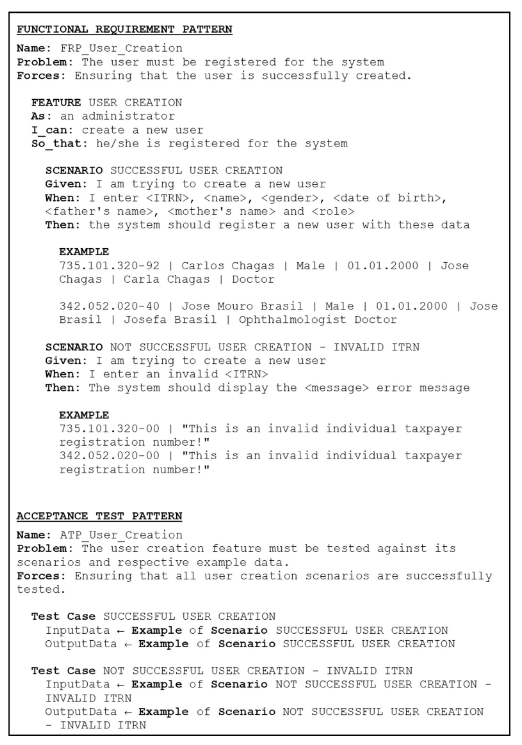
\includegraphics[width=15cm]{img/metamodelo.png}
	\caption{La estructura y los con-tentos de un FRP asociado a un ATP.}
	\label{fig:metamodelo}
\end{figure}

Como se observa en la figura \ref{fig:metamodelo_sopamm} FRP\_User\_Creation describe una parte de la función para crear usuarios. Se puede visualizar que el usuario administrador es el actor beneficiado de esta función para que se logre registrar un nuevo usuario al sistema. El intento de crear un usuario conlleva a dos posibles escenarios: uno exitoso y otro no exitoso, pero ambos vinculados a una misma precondición.  Sin embargo, dependiendo de la validez de los usuarios la ejecución puede ser distinta. Del mismo modo por cada escenario se representara un resultado diferente, es decir se visualizaran mensajes diferentes al momento de registrar un usuario o mensajes de error [2].

Finalmente el ejemplo mostrado permite definir y vincular varios datos cada escenario. En cada escenario se consta con dos instancias de datos, de manera que uno de los escenarios registrado un nuevo usuario con éxito, mientras que el otro no lo hace debido a que los datos de entrada no son validos, como es el numero de identificación del usuario. Esta representación define el enfoque de patrones de requisitos funcionales basado en el comportamiento de los posibles escenarios. En la figura \ref{fig:metamodelo_sopamm} se observa el metamodelo de SoPaMM [2].

\begin{figure}[h!]
	\centering
	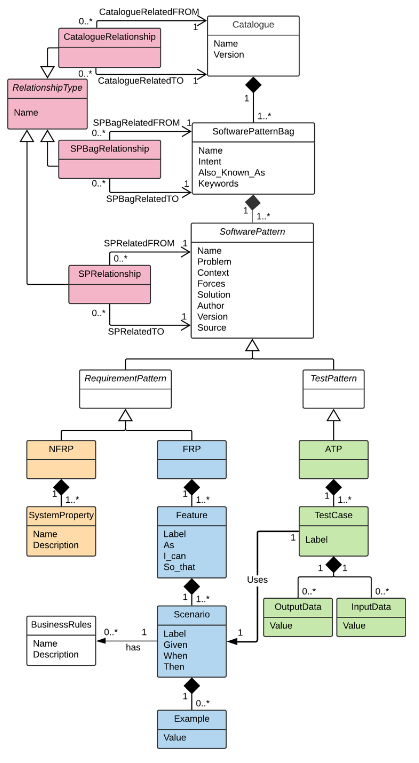
\includegraphics[width=10cm]{img/metamodelosopamm.png}
	\caption{El metamodelo SoPaMM.}
	\label{fig:metamodelo_sopamm}
\end{figure}


\subsection{Desarrollo ágil de software}

El desarrollo ágil de software hace referencia a los principios del manifiesto ágil que son aplicadas por varias metodologías de desarrollo. Las metodologías de desarrollo ágil comparten varias características como: la entrega frecuente de software de trabajo (desarrollo iterativo), la velocidad constante y la comunicación abierta [5]. En el desarrollo ágil los métodos que se emplean pueden ser de bajo costo, es decir que cualquier modificación que se realice en alguna etapa de desarrollo el cliente podrá observar los resultados deseados referente al costo que ha pagado [6]. 

Ademas de ser una buena alternativa para mejorar el desarrollo de software, el desarrollo ágil es muy productivo por que brecha de comunicación entre los clientes y los desarrolladores de software. Conforme avance el tiempo, difícilmente pueden surgir motivos para generar retrasos. Lo beneficioso de aplicar este proceso es que los cambios pueden ser acoplados continuamente de acuerdo a las necesidades del cliente. A continuación se mencionaran varias metodologías ágiles que se utilizan en el desarrollo de software [6]:

\begin{itemize}
	\item \textbf{La programación extrema (XP) :} Esta es una metodología centrada específicamente en obtener un software de calidad. Para cumplir con ese objetivo, se debe considerar en primer lugar una buena comunicación verbal entre todos los integrantes del proyecto. Ademas no existen reglas que obliguen a llevar una documentación rigurosa, con el fin de aumentar la eficiencia de desarrollo del software.
	
	\item \textbf{Dynamic Systems Development Method (DSDM): }En DSDM o en su traducción al español Sistemas dinámicos Método de desarrollo la documentacion es totalmente necesaria, debe ser magra y oportuna describiendo paso a paso todo el proceso que se realizo. Esto significa que el modelo y el prototipo deberán representar una visión general sobre lo que va hacer el sistema. Ademas se deberán documentar los diagramas de modelado, estructuras físicas de datos y decisiones de diseño.
	
	\item \textbf{Scrum: } Se centra netamente en la versatilidad rentabilidad y adaptabilidad. Le permite al desarrollador tomar la decisión para elegir la técnica de ejecución del modulo que este encargado. La administración de Scrum permite reconocer las carencias u obstáculos que se presentaran a lo largo del proyecto. Los equipos de Scrum tiene la libertad de elegir y reconocer los enfoques para realizar su trabajo, es decir que cada integrante del grupo cuanta con las habilidades necesarias para cumplir su trabajo sin necesidad de recurrir a pedir ayuda fuera del grupo.
\end{itemize}



